\documentclass{article}
\usepackage[margin=1in]{geometry}
\usepackage{amsmath}
\usepackage{amssymb}
\usepackage{amsthm}
\usepackage{url}
\usepackage{todonotes}
\usepackage{svg}
\usepackage{cleveref}

% Environments

\newtheorem{theorem}{Theorem}
\newtheorem{proposition}[theorem]{Proposition}
\newtheorem{corollary}[theorem]{Corollary}
\newtheorem{lemma}[theorem]{Lemma}
\newtheorem{definition}[theorem]{Definition}
\newtheorem{conjecture}[theorem]{Conjecture}
\newtheorem{remark}[theorem]{Remark}


\theoremstyle{definition}
\newtheorem{example}[theorem]{Example}

\numberwithin{theorem}{section}
\numberwithin{equation}{section}

\DeclareMathOperator{\Int}{int}
\DeclareMathOperator{\Star}{st}
\DeclareMathOperator{\Lk}{lk}
\DeclareMathOperator{\Homeo}{Homeo}
\newcommand{\atlas}{\mathcal{A}}
\newcommand{\cover}{\widetilde{X}}

%opening
\title{Low Dimensional Topology}
\author{Eric Luu}

\begin{document}
\section{11}
\setkeys{Gin}{width=1cm}
\newcommand{\RIIcross}{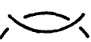
\includegraphics{Figures/Crossings/R2cross.png}}
\newcommand{\RIIItop}{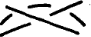
\includegraphics{Figures/Crossings/R3top.png}}
\newcommand{\RIIIbottom}{\raisebox{5pt}{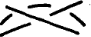
\includegraphics[angle = 180]{Figures/Crossings/R3top.png}}}
\newcommand{\Kcross}{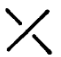
\includegraphics[width = 0.5cm]{Figures/Crossings/crossing.png}}
\newcommand{\Kcrossreflect}{\reflectbox{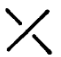
\includegraphics[width = 0.5cm]{Figures/Crossings/crossing.png}}}

\newcommand{\ARes}{\raisebox{-5pt}{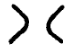
\includegraphics[width = 0.8cm]{Figures/Crossings/A_res.png}}}
\newcommand{\BRes}{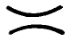
\includegraphics[width = 0.5cm]{Figures/Crossings/B_res.png}}
\newcommand{\plusOne}{\includesvg[width = 0.5cm]{Figures/Crossings/arrow_crossing.svg}}
\newcommand{\minusOne}{\reflectbox{\includesvg[width = 0.5cm]{Figures/Crossings/arrow_crossing.svg}}}


\subsection{4}

Firstly, $P$ is always invariant under ambient isotopy. When the knot diagram is moved around, the crossings do not change and the underlying $4$-valent graphs stay the same. Therefore, the properties of $P$ are the same.  

If $P$ is invariant under Reidermeister II moves and ambient isotopy, $P$ is invariant under Reidermeister III moves. 

This is because of the following:
\begin{align*}
    P(\RIIItop) &= f(A)P(\raisebox{-5pt}{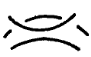
\includegraphics{Figures/Crossings/R3Ares.png}}) + g(A)P(\raisebox{-5pt}{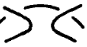
\includegraphics{Figures/Crossings/R3Bres.png}})\\
    &= f(A)P(\raisebox{10pt}{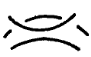
\includegraphics[angle = 180]{Figures/Crossings/R3Ares.png}}) + g(A)P(\raisebox{10pt}{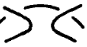
\includegraphics[angle = 180]{Figures/Crossings/R3Bres.png}})\\
    &=P(\RIIIbottom)
\end{align*}
where the third step comes from applying Reidermeister II moves and the ambient isotopy relation.


Now $P$ is invariant under Reidermeister II moves if and only if $fg = 1$ and $h = -f^2 - g^2$. 

\begin{align*}
    P(\RIIcross) &= f(A)P(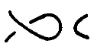
\includegraphics{Figures/Crossings/R2Ares.png}) + g(A) P(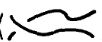
\includegraphics{Figures/Crossings/R2Bres.png})\\
    &= f(A)\left(f(A)P(\ARes) + g(A) P(\raisebox{-5pt}{\includesvg[width = 0.8cm]{Figures/Crossings/R2djcircle.svg}})\right) + g(A)\left(f(A) P(\BRes) + g(A)P(\ARes)\right)\\
    &=f(A)\left(f(A)P(\ARes) + g(A) h(A) P(\ARes)\right) + g(A)\left(f(A) P(\BRes) + g(A)P(\ARes)\right)\\
    &= g fP(\BRes) +(f^2 + fgh + g^2) P(\ARes)
\end{align*}

Since $P$ is a polynomial,$g fP(\BRes) +(f^2 + fgh + g^2) P(\ARes) = P(\BRes)$ if and only if $gf = 1$ and $f^2 + h + g^2 = 0$. Then $h = -f^2 - g^2$.

Therefore, $P$ is invariant under ambient isotopy, Reidermeister II and III moves if and only if $fg = 1$ and $h = -f^2 - g^2$. 


\subsection{6}

We want to show that \[(-A)^{-3w(L^*)}\langle L^* \rangle(A) = (-A)^{3w(L)}\langle L \rangle(A^{-1}).\] If this is the case, then substituting $t^{1/2} = A^{-2}$ yields $V(L^*)(t) = V(L)(t^{-1})$. 

Firstly, $w(L^*) = -w(L)$. This is because for every crossing, \plusOne, which is $+1$ writhe becomes \minusOne, which is $-1$ writhe. 

Next, $\langle L^* \rangle(A) = \langle L \rangle(A^{-1})$. We prove this by induction.
For the base case, if $L$ is the unknot, the $L^*$ is also the unknot so $\langle L^* \rangle(A) = \langle L \rangle(A^{-1}) = 1$. If there is a disjoint unknot, then flipping the link keeps the unknot disjoint. Assume for the induction hypothesis that $\langle L^* \rangle(A) = \langle L \rangle(A^{-1})$, and the knot we are working with is $L \sqcup O$. Then
\[\langle L \sqcup O \rangle(A^{-1}) = (-A^2 - A^{-2}) \langle L \rangle(A^{-1}) = (-A^2 - A^{-2}) \langle L^* \rangle(A) = \langle O \sqcup L^* \rangle(A).\]
This is because $(-A^2 - A^{-2})$ is symmetric when $A \mapsto A^{-1}$.

Finally,  \[\langle \Kcross \rangle(A^{-1}) = A^{-1} \langle \ARes \rangle(A^{-1}) + A \langle \BRes \rangle(A^{-1}).\] By induction, \[\langle \ARes \rangle(A^{-1}) = \langle \ARes^* \rangle(A)\]
and  \[\langle \BRes \rangle(A^{-1}) = \langle \BRes^* \rangle(A).\]
But if $L$ has \Kcross, then \Kcross becomes \Kcrossreflect in $L^*$. So in $L^*$, \ARes and \BRes are swapped, so \[\langle \Kcrossreflect \rangle(A) = A \langle \BRes^* \rangle(A) + A^{-1} \langle \ARes^* \rangle(A) = A \langle \BRes \rangle(A^{-1}) + A^{-1} \langle \ARes \rangle(A^{-1}) = \langle \Kcross \rangle(A^{-1}).\] Therefore, $\langle L^* \rangle(A) = \langle L \rangle(A^{-1})$. Finally, $(-A)^{-3w(L^*)}\langle L^* \rangle(A) = (-A)^{3w(L)}\langle L \rangle(A^{-1})$, so $V(L^*)(t) = V(L)(t^{-1})$. 

\subsection{7}
Exercise 6 implies that if a knot $K$ is amphichiral, then $V(K)(t) = V(K)(t^{-1})$. 

The right trefoil has Jones polynomial $-t^4 + t^3 + t$, from Lickorish (p 29). By exercise 6,  $t \mapsto t^{-1}$ is the Jones polynomial of the left trefoil, which is $-t^{-4} + t^{-3} + t^{-1}$. Therefore, the trefoil is not amphichiral.

\subsection{8}

First, we want to show that $w(K_1 \# K_2) = w(K_1) + w(K_2)$ and $\langle K_1 \# K_2 \rangle = \langle K_1 \rangle\langle K_2 \rangle$. If this holds, then \[(-A)^{-3w(K_1 \# K_2)} \langle K_1 \# K_2 \rangle = (-A)^{-3w(K_1)} \langle K_1 \rangle (-A)^{-3w(K_2)} \langle K_2 \rangle,\] which implies that $V(K_1 \# K_2) = V(K_1) V(K_2)$ by setting $t^{1/2} = A^{-2}$. 

Firstly, $w(K_1 \# K_2) = w(K_1) + w(K_2)$ since every crossing in $w(K_1 \# K_2)$ is either in $K_1$ or $K_2$, so the writhe number is additive. 

We have from the sum of states formula that:
\[\langle K_1 \# K_2\rangle = \sum_{s}\left[A^{d(s)}(-A^2 - A^{-2})^{|s| - 1} \right],\] where $d(s)$ is the sum of $A - B$ turns for each crossing and $|s|$ are the number of disjoint circles at the end. 

We can decompose every state $s$ into two substates $s_1, s_2$ where $s_1$ are on crossings in $K_1$ and $s_2$ are on crossings in $K_2$. Each $s_1$ is paired with an $s_2$ to form all $s$, and in fact every combination of $s_1$ and $s_2$ appears exactly once. Secondly, since $d(s)$ counts the number of $A - B$ crossings, $d(s) = d(s_1) + d(s_2)$. Finally, the number of disjoint circles of $s_1$ and $s_2$ is equal to $s$ except that two circles, one from $K_1$ and one from $K_2$ are linked together from the connected sum operation. Then $|s| = |s_1| + |s_2| - 1$. So

\begin{align*}
    \langle K_1 \# K_2\rangle &= \sum_{s}\left[A^{d(s)}(-A^2 - A^{-2})^{|s| - 1} \right]\\
    &= \sum_{s_1 + s_2}\left[A^{d(s_1) + d(s_2)}(-A^2 - A^{-2})^{|s_1|- 1 + |s_2| - 1} \right]\\
    &= \sum_{s_1 + s_2}\left[A^{d(s_1)}(-A^2 - A^{-2})^{|s_1|- 1} \right] \left[A^{d(s_2)}(-A^2 - A^{-2})^{|s_2|- 1} \right]\\
    &= \sum_{s_1}\left[A^{d(s_1)}(-A^2 - A^{-2})^{|s_1|- 1} \right] \sum_{s_2}\left[A^{d(s_2)}(-A^2 - A^{-2})^{|s_2|- 1} \right]\\
    &= \langle K_1 \rangle \langle K_2 \rangle
\end{align*}
Therefore,  $V(K_1 \# K_2) = V(K_1) V(K_2)$.
\end{document}
